\documentclass[12pt]{report}
\usepackage{lingmacros}
\usepackage{tree-dvips}
\usepackage{graphicx}
\usepackage{listings}
\graphicspath{ {images/} }

\begin{document}

\section*{Report Labwork XI}

\subsection*{I: How you made up the structure}


Explain:
{\small
\enumsentence{Offices and directors: one to one. But they need to split into 2 tables, because they are two entity}}

{\small
\enumsentence{Offices and projects: one to many. One offices can have many project and maybe one project can have many office co-op}}

{\small
\enumsentence{Projects and managers: many to one. Manager can have many project, and project can change their manager, so project also have many manager}}

{\small
\enumsentence{offices and cities: many to one. Each office locate in only one city, and each city belong to only one country. But one country can have many cities}}

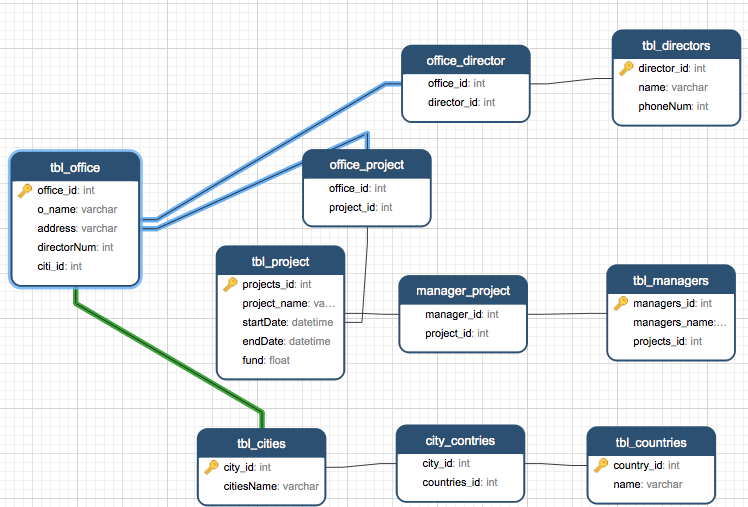
\includegraphics[width=0.7\paperwidth]{lab11}




\subsection*{II: SQL commands to create the database}

\textbf {Create database}

Create database labwork11 
\begin{lstlisting}[language=sql]

CREATE DATABASE labwork11;

\end{lstlisting}
Output: Query OK, 0 rows affected (0.00 sec)

\textbf {Disable FOREIGN KEY CHECKS}

Disable Foreign key check to create foreign key in tables
 
\begin{lstlisting}[language=sql]

SET FOREIGN_KEY_CHECKS = 0;

\end{lstlisting}
Output: Query OK, 0 rows affected (0.00 sec)

---------------------------------------------------------------



CREATE Table structure for `city\_contries`

\begin{lstlisting}[language=sql]
CREATE TABLE `city_contries` (
  `city_id` int(11) DEFAULT NULL,
  `countries_id` int(11) DEFAULT NULL,
  KEY `city_id` (`city_id`),
  KEY `countries_id` (`countries_id`)
)
\end{lstlisting}
Output: Query OK, 0 rows affected (0,00 sec)0,00
CREATE Table structure for `manager\_project`

\begin{lstlisting}[language=sql]
CREATE TABLE `manager_project` (
  `manager_id` int(11) DEFAULT NULL,
  `project_id` int(11) DEFAULT NULL,
  KEY `project_id` (`project_id`),
  KEY `manager_id` (`manager_id`)
)
\end{lstlisting}
Output: Query OK, 0 rows affected (0,00 sec)
CREATE Table structure for `office\_director`

\begin{lstlisting}[language=sql]
CREATE TABLE `office_director` (
  `office_id` int(11) DEFAULT NULL,
  `director_id` int(11) DEFAULT NULL,
  KEY `office_id` (`office_id`),
  KEY `director_id` (`director_id`)
)
\end{lstlisting}
Output: Query OK, 0 rows affected (0,00 sec)
CREATE Table structure for `office\_project`

\begin{lstlisting}[language=sql]
CREATE TABLE `office_project` (
  `office_id` int(11) DEFAULT NULL,
  `project_id` int(11) DEFAULT NULL,
  KEY `office_id` (`office_id`),
  KEY `project_id` (`project_id`)
)
\end{lstlisting}
Output: Query OK, 0 rows affected (0,00 sec)
CREATE Table structure for `tbl\_cities`

\begin{lstlisting}[language=sql]
CREATE TABLE `tbl_cities` (
  `city_id` int(11) NOT NULL,
  `citiesName` varchar(255) DEFAULT NULL,
  PRIMARY KEY (`city_id`),
  CONSTRAINT `city` FOREIGN KEY (`city_id`) REFERENCES `city_contries` (`city_id`) ON DELETE CASCADE ON UPDATE CASCADE,
  CONSTRAINT `city2` FOREIGN KEY (`city_id`) REFERENCES `tbl_office` (`citi_id`) ON DELETE CASCADE ON UPDATE CASCADE
)
\end{lstlisting}
Output: Query OK, 0 rows affected (0,00 sec)
CREATE Table structure for `tbl\_countries`

\begin{lstlisting}[language=sql]
CREATE TABLE `tbl_countries` (
  `country_id` int(11) NOT NULL AUTO_INCREMENT,
  `name` varchar(255) DEFAULT NULL,
  PRIMARY KEY (`country_id`),
  CONSTRAINT `contries` FOREIGN KEY (`country_id`) REFERENCES `city_contries` (`countries_id`) ON DELETE CASCADE ON UPDATE CASCADE
)
\end{lstlisting}
Output: Query OK, 0 rows affected (0,00 sec)
CREATE Table structure for `tbl\_directors`

\begin{lstlisting}[language=sql]
CREATE TABLE `tbl_directors` (
  `director_id` int(11) NOT NULL AUTO_INCREMENT,
  `name` varchar(255) DEFAULT NULL,
  `phoneNum` int(11) DEFAULT NULL,
  PRIMARY KEY (`director_id`),
  CONSTRAINT `director` FOREIGN KEY (`director_id`) REFERENCES `office_director` (`director_id`) ON DELETE CASCADE ON UPDATE CASCADE
)
\end{lstlisting}
Output: Query OK, 0 rows affected (0,00 sec)
CREATE Table structure for `tbl\_managers`

\begin{lstlisting}[language=sql]
CREATE TABLE `tbl_managers` (
  `managers_id` int(11) NOT NULL AUTO_INCREMENT,
  `managers_name` varchar(255) DEFAULT NULL,
  `projects_id` int(11) DEFAULT NULL,
  PRIMARY KEY (`managers_id`),
  CONSTRAINT `manager` FOREIGN KEY (`managers_id`) REFERENCES `manager_project` (`manager_id`) ON DELETE CASCADE ON UPDATE CASCADE
)
\end{lstlisting}
Output: Query OK, 0 rows affected (0,00 sec)
CREATE Table structure for `tbl\_office`

\begin{lstlisting}[language=sql]
CREATE TABLE `tbl_office` (
  `office_id` int(11) NOT NULL AUTO_INCREMENT,
  `o_name` varchar(255) DEFAULT NULL,
  `address` varchar(255) DEFAULT NULL,
  `directorNum` int(11) DEFAULT NULL,
  `citi_id` int(11) DEFAULT NULL,
  PRIMARY KEY (`office_id`),
  KEY `citi_id` (`citi_id`),
  CONSTRAINT `office` FOREIGN KEY (`office_id`) REFERENCES `office_director` (`office_id`) ON DELETE CASCADE ON UPDATE CASCADE,
  CONSTRAINT `office2` FOREIGN KEY (`office_id`) REFERENCES `office_project` (`office_id`) ON DELETE CASCADE ON UPDATE CASCADE
)
\end{lstlisting}
Output: Query OK, 0 rows affected (0,00 sec)
CREATE Table structure for `tbl\_project`

\begin{lstlisting}[language=sql]
CREATE TABLE `tbl_project` (
  `projects_id` int(11) NOT NULL AUTO_INCREMENT,
  `project_name` varchar(255) DEFAULT NULL,
  `startDate` datetime DEFAULT NULL,
  `endDate` datetime DEFAULT NULL,
  `fund` float DEFAULT NULL,
  PRIMARY KEY (`projects_id`),
  CONSTRAINT `project` FOREIGN KEY (`projects_id`) REFERENCES `manager_project` (`project_id`) ON DELETE CASCADE ON UPDATE CASCADE,
  CONSTRAINT `project2` FOREIGN KEY (`projects_id`) REFERENCES `office_project` (`project_id`) ON DELETE CASCADE ON UPDATE CASCADE
)
\end{lstlisting}
Output: Query OK, 0 rows affected (0,00 sec)


-----------------------------------------------------------------------

\textbf {Enable FOREIGN KEY CHECKS}

Enable Foreign key check
 
\begin{lstlisting}[language=sql]

SET FOREIGN_KEY_CHECKS = 1;
\end{lstlisting}

Output: Query OK, 0 rows affected (0.00 sec)

-------------------------------------------------------------------------

\end{document}